\documentclass[../rapport_MVEX01-11-05]{subfiles}
\begin{document}

\subsection{$k$-nearest-neighbour}

%Detta måste givetvis göras en gång per gest, vilket ger oss en kodbok
%per gest; detta eftersom vi har en HMM per gest.
%
%\marginpar{Eller, hur ska vi göra egentligen? En eller flera
% kodböcker? Hur skalar algoritmerna, hur jobbigt blir det? Säger
% någon referens något om detta?}

%FIGUR
%http://en.wikipedia.org/wiki/File:KnnClassification.svg
\begin{figure}[!htpb]
    \begin{center}
%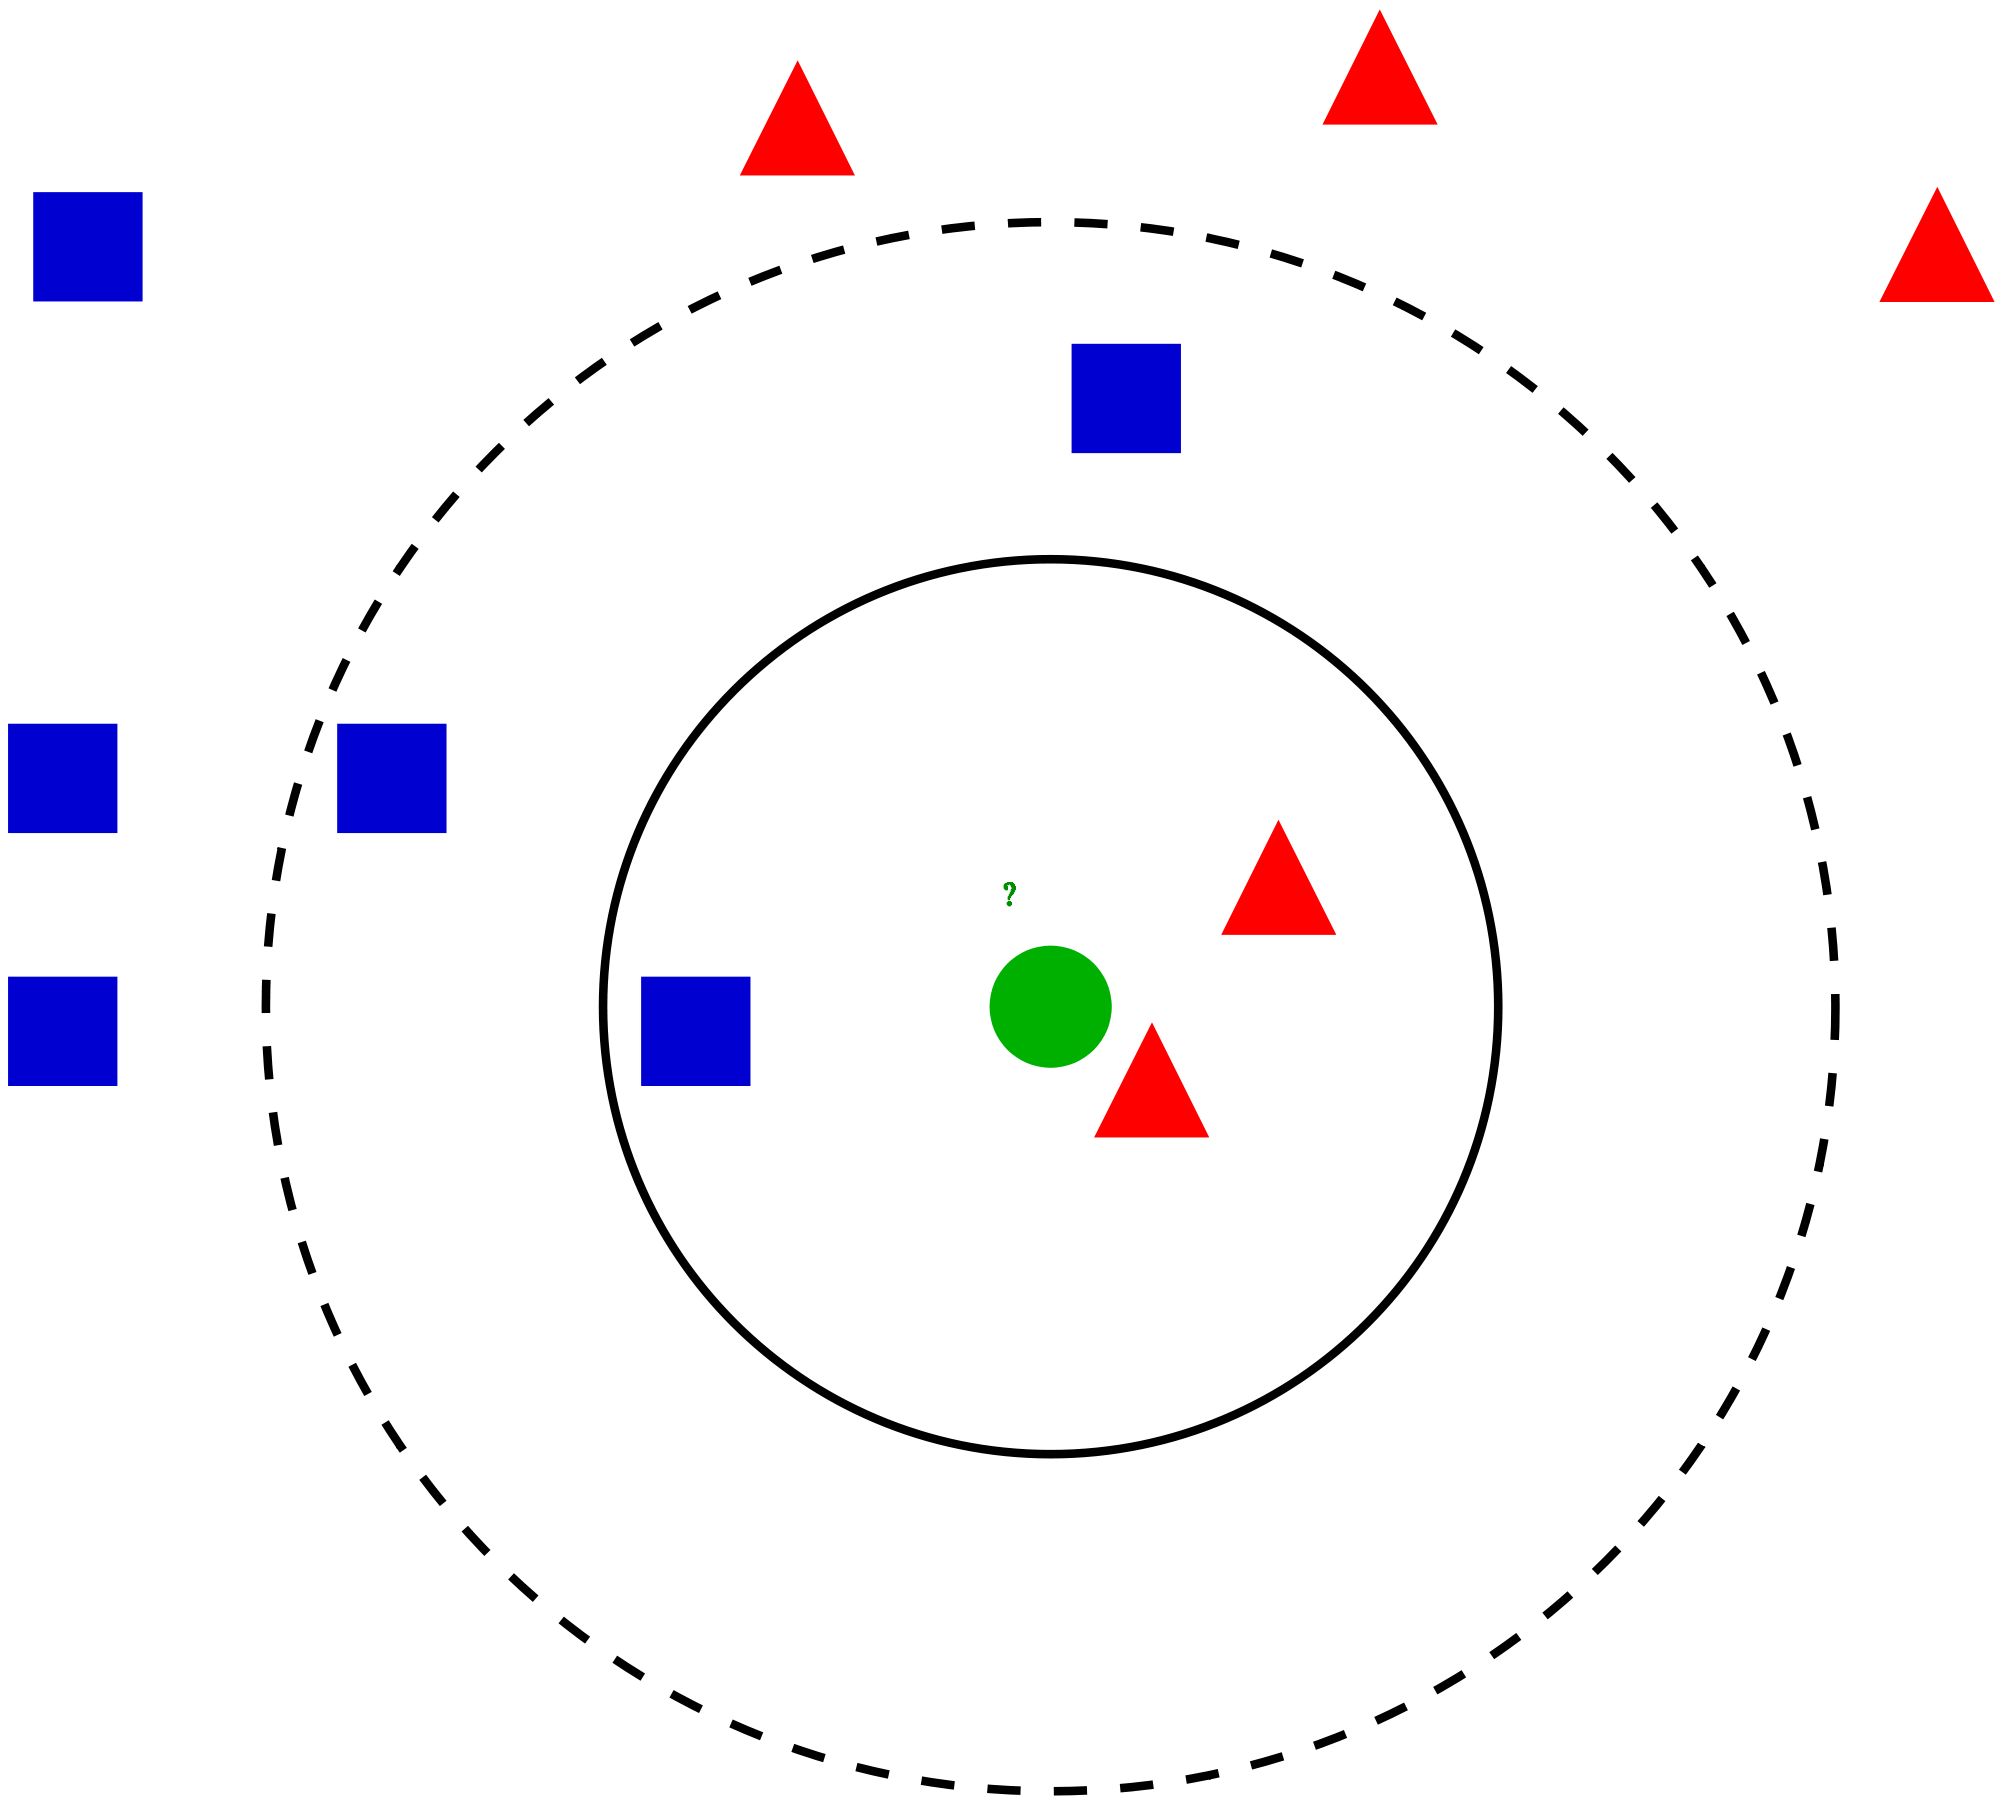
\includegraphics[width=\columnwidth]{bilder/2000px-KnnClassification.jpg}
    \end{center}
    \caption{kNN-klassificering av den runda observationen i mitten i ett rum
    med två klasser, trianglar och kvadrater. Majoritetsomröstning
    med $k=3$ leder till att den runda klassas som triangel, medan $k=5$ leder
    till klassificering som kvadrat. \copyright Antti Ajanki, 2007}
    \label{fig:knn-overview}
\end{figure}

\end{document}